% FIRST DRAFT, not for circulation.  Theory of the relative GLV economy with demographic noise and
% firm turnover.  Numbers come from scripts/demographic/ (outputs in data/demographic/, gitignored);
% figures from scripts/demographic/paper_figures.py.  Build: latexmk -pdf demographic.tex
\documentclass[pre,twocolumn,superscriptaddress,nofootinbib]{revtex4-2}
\usepackage{amsmath,amssymb,bm}
\usepackage{graphicx}
\usepackage{booktabs}
\graphicspath{{../../assets/figures/}}
\usepackage[hidelinks]{hyperref}

\newcommand{\E}{\mathbb E}
\newcommand{\Var}{\operatorname{Var}}
\newcommand{\Sb}{\bar S}
\newcommand{\todo}[1]{\textbf{[#1]}}

\begin{document}

\title{Demographic noise and the size--volatility law in a Lotka--Volterra economy}
\author{Ludovico Furlanetto}
\date{First draft, \today}

\begin{abstract}
We add demographic noise and firm turnover to a scale-invariant generalised Lotka--Volterra
model of interacting firms.  A firm that reaches zero size is replaced by a newborn of one unit,
which removes the immigration floor and the listing threshold of the deterministic model while
keeping the number of parameters fixed.  We show numerically that each firm then behaves as a
single logistic unit driven by its own field plus its own noise, and that at constant field this
one-firm problem is solved by quadratures.  With turnover a node is a renewal process with an exact
stationary law, and a static cavity theory built on it gives the instability line $\sigma_c(D)$, which
reduces to the deterministic line as $D\to0$ and rises with the noise, and predicts the turnover rate
to within $0.5\%$.  The growth volatility of a firm over its life is the
sum of a fitness part, nearly independent of size, and a demographic part, filtered by the firm's
own relaxation, which falls as the inverse size.  The size--volatility relation is therefore a
crossover from slope $-1/2$ to slope $0$.  At one reference point (degree tail $\alpha=2.5$)
the crossover is nearly straight over two decades, with an effective exponent
$\beta\simeq0.16$--$0.20$ and a multiscaling ratio curve close to the Compustat values.  The same
logistic plateau that produces the law caps firm size, so the model has no Pareto tail, and it
has unrealistic infant mortality.  We read the size--volatility exponent as an effective exponent
of a crossover rather than a scaling law.
\end{abstract}

\maketitle

%======================================================================
\section{Introduction}

The growth rates of large firms fluctuate less than those of small firms.  If $v$ is the
volatility of a firm's growth rate and $\Sb$ its mean size, the conditional moments behave as
$\E[v^q\mid\Sb]\sim\Sb^{-\zeta_q}$ with $\beta=\zeta_1\approx0.15$--$0.2$
\cite{stanley1996,amaral1997,sutton2002}, and the ratios $\zeta_q/\zeta_1\approx2.0,\,2.6,\,2.9$ for
$q=2,3,4$ fall below the line $\zeta_q/\zeta_1=q$ \cite{moran2024}.  Whether this is a scaling law is
disputed.  Moran, Secchi and Bouchaud \cite{moran2024} fit one exponent over about four decades of
Compustat firms.  Fontanelli, Napoletano and Secchi \cite{fontanelli2025}, conditioning on current
size in French data that include very small firms, find two regimes instead: a slope near $-0.5$
for small firms and a nearly flat relation above a crossover close to half the median firm.

In earlier work we studied a generalised Lotka--Volterra (GLV) economy in which interactions are
measured in units of the mean firm, so that the economy grows at a self-consistent rate while
its composition follows a disordered replicator.  A deterministic immigration floor $\lambda$
kept firms from vanishing.  Under the unbalanced panel used for firm data that model gives a
humped size--volatility curve: firms near the floor are calm, and volatility falls only over the
top decade of sizes.

Here we replace the floor by the stochastic ingredient that population models usually carry,
demographic noise, together with a turnover rule.  The change is small and keeps the parameter
count, but it changes the size--volatility relation qualitatively.  Our results are:
\begin{enumerate}
\item each firm is a logistic unit driven by its measured field and its own noise, to the
  accuracy of the simulations (Sec.~\ref{sec:reduction});
\item at constant field the one-firm problem is a one-dimensional diffusion with exact
  establishment probabilities, extinction times and, with turnover, an exact renewal law
  (Sec.~\ref{sec:constant});
\item a static cavity theory built on the renewal law gives the phase diagram in the plane of
  disorder and noise: the instability line rises with $D$ from its deterministic value, and the
  turnover rate is predicted to within $0.5\%$ (Sec.~\ref{sec:phase});
\item a firm's growth variance over its life is a fitness part plus a filtered demographic part,
  predicted to about $5\%$ across sizes, and the size--volatility relation is the crossover
  between them (Sec.~\ref{sec:law});
\item at a reference point the life panel gives $\beta\simeq0.2$ with a near-data ratio curve, while
  the size distribution, the infant mortality and the growth-rate skewness are wrong for a
  structural reason (Secs.~\ref{sec:panel} and \ref{sec:limits}).
\end{enumerate}

%======================================================================
\section{Model}
\label{sec:model}

\paragraph{Absolute form.}  Firm $i=1,\dots,N$ has size $x_i$ and sits on a node of a power-law
configuration graph with degree tail $P(k)\sim k^{-\alpha}$ and mean degree $C$.  With $m=\sum_ix_i/N$
the mean firm,
\begin{equation}
dx_i=x_i\Big(1-\frac{x_i}{m}-\sum_ja_{ij}\frac{x_j}{m}\Big)dt+\sqrt{D\,m\,x_i}\;dW_i ,
\label{eq:abs}
\end{equation}
with independent Wiener processes $W_i$.  This is the GLV equation with unit growth rate,
carrying capacity equal to the mean firm, interactions measured in units of the mean firm, and
the birth--death noise of stochastic Lotka--Volterra models \cite{altieri2021} with unit $Dm$.
On each edge the couplings are independent Gaussians with mean $\mu/C$ and standard deviation
$\sigma/\sqrt C$, with $C$ the realised mean degree (no reciprocity); $\mu>0$ is net competition.  A firm that reaches $x_i=0$ exits, and a newborn of size $Dm$
takes its node and its couplings: a new firm in the same niche.

\paragraph{Relative form.}  With $S_i=x_i/m$, so that $\sum_iS_i=N$,
\begin{equation}
dS_i=S_i\,(f_i-\bar f)\,dt+\sqrt{DS_i}\,dW_i-\frac{S_i}{N}\sum_j\sqrt{DS_j}\,dW_j ,
\label{eq:rel}
\end{equation}
where $f_i=1-S_i-\sum_ja_{ij}S_j$ and $\bar f=\sum_iS_if_i/N$ is the growth rate of the mean firm.  The
last term, of order $N^{-1/2}$, keeps $\sum_iS_i=N$.  Exit is at $S_i=0$ and entry at $S_i=D$.  The
parameters are $\mu,\sigma,\alpha,C$ and $D$; $D$ replaces the floor $\lambda$ of the deterministic
model.

\paragraph{Numerics and protocol.}  We integrate Eq.~\eqref{eq:rel} by Euler--Maruyama with step
$0.01$ (\texttt{relative\_glv.model.integrate\_demographic}), discard $t<100$ and record sizes
every $\Delta t=0.5$ for a window of $480$.  Growth rates are $g=\Delta\ln S$ over $\Delta t$.  A
\emph{life} runs from a birth to the next exit at the same node; lives cut by the window are kept,
as in an unbalanced panel.  A life's volatility is $v=\sqrt{\pi/2}$ times the mean absolute
deviation of its growth rates around their own mean, $\Sb$ is its mean size, and lives need at
least $n_{\min}$ growth rates.  Exponents $\zeta_q$ are least-squares slopes of $\ln\E[v^q\mid\Sb]$ over
$25$ equal-count bins of $\Sb$, all bins included \cite{moran2024}.  Unless stated, $\mu=1.76$,
$C=200$ and $N=8000$, with eight economies per point.

%======================================================================
\section{One-firm reduction}
\label{sec:reduction}

Define the field of firm $i$,
\begin{equation}
\Phi_i(t)=1-\sum_ja_{ij}S_j(t)-\bar f(t).
\end{equation}
Equation~\eqref{eq:rel} is then, up to the $O(N^{-1/2})$ term,
\begin{equation}
dS_i=S_i\,(\Phi_i-S_i)\,dt+\sqrt{DS_i}\,dW_i ,\qquad S_i=0\to S_i=D .
\label{eq:onefirm}
\end{equation}
This is an identity.  Its content is that the field can be treated as given: a firm's own noise
should not feed back on its field through the network.  We test this directly.  We store the
fields of two full economies at $\alpha=2.5$, $\sigma=1.75$, $D=0.1$, integrate
Eq.~\eqref{eq:onefirm} for every node with its measured $\Phi_i(t)$ and fresh noise, and compare the
life panels (Table~\ref{tab:reduction}, Fig.~\ref{fig:reduction}).  Exponents agree to $0.01$, ratios
to $0.05$ and exit rates to $2\%$.  For the rest of the paper the theory is the one-firm problem
\eqref{eq:onefirm} with a field $\Phi(t)$ whose statistics come from the network.

\begin{table}[b]
\caption{Full model against one firm in its measured field (two economies, $\alpha=2.5$,
$\sigma=1.75$, $D=0.1$, $N=8000$).  Source: \texttt{scripts/demographic/reduction.py}.}
\label{tab:reduction}
\begin{ruledtabular}
\begin{tabular}{lcccc}
$n_{\min}$ & $\beta$ full & $\beta$ one firm & $\zeta_q/\zeta_1$ full & $\zeta_q/\zeta_1$ one firm\\
\hline
2  & 0.198 & 0.203 & 2.45, 4.10, 5.82 & 2.44, 4.08, 5.81\\
10 & 0.294 & 0.306 & 1.82, 2.44, 2.90 & 1.83, 2.46, 2.95\\
20 & 0.376 & 0.388 & 1.82, 2.40, 2.76 & 1.83, 2.43, 2.81\\
\end{tabular}
\end{ruledtabular}
\end{table}

\begin{figure}[t]
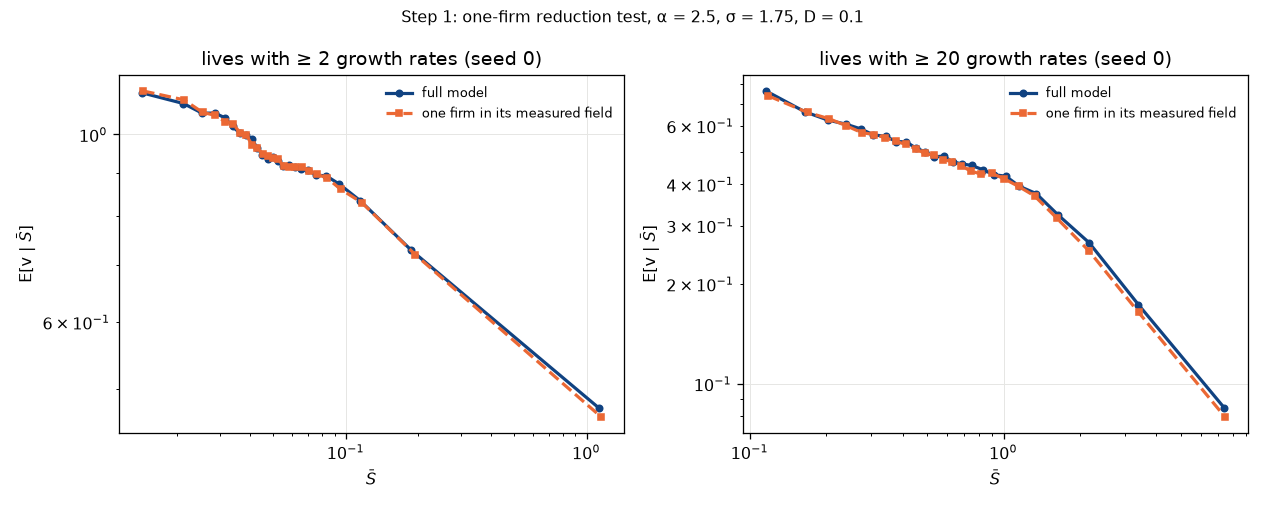
\includegraphics[width=\linewidth]{demographic_reduction.png}
\caption{Life-panel volatility of the full model and of independent firms driven by their measured
fields (economy 0 of Table~\ref{tab:reduction}).}
\label{fig:reduction}
\end{figure}

%======================================================================
\section{Constant field}
\label{sec:constant}

At constant $\Phi$, Eq.~\eqref{eq:onefirm} is a one-dimensional diffusion with drift $b(S)=S(\Phi-S)$
and diffusion coefficient $DS$, absorbed at $0$.  Its scale density is
\begin{equation}
s'(y)=\exp\Big[-\frac2D\Big(\Phi y-\frac{y^2}{2}\Big)\Big],
\end{equation}
and the standard formulas for one-dimensional diffusions \cite{karlintaylor1981} give everything
about entry and exit in closed form.

\paragraph{Establishment.}  A newborn reaches its plateau $S=\Phi$ before exiting with probability
\begin{equation}
P_{\rm est}(\Phi)=\frac{\int_0^Ds'(y)\,dy}{\int_0^\Phi s'(y)\,dy}\qquad(\Phi>D).
\label{eq:pest}
\end{equation}
Dropping the logistic term gives the Feller estimate $1-e^{-2\Phi}$, which is off by up to
$0.2$ at $D=0.1$.

\paragraph{Exit time.}  The mean time to exit from $S_0$ is
\begin{equation}
T(S_0)=2\int_0^{S_0}s'(y)\int_y^\infty\frac{dz}{Dz\,s'(z)}\,dy .
\label{eq:text}
\end{equation}
For $\Phi\le0$ it is of order $1/|\Phi|$ and, for a newborn, independent of $D$: near zero the logistic term
is negligible and the Feller survival probability from $S_0=D$, $1-\exp[-2|\Phi|/(e^{|\Phi|t}-1)]$, does not
contain $D$.
For $\Phi>0$ it grows as $e^{\Phi^2/D}$ at large $\Phi^2/D$, the quasi-potential of the plateau, so an
established firm with $\Phi\sim1$ exits through dips of its field rather than through noise.
Table~\ref{tab:constant} compares Eqs.~\eqref{eq:pest} and \eqref{eq:text} with direct simulation.

\begin{table}[b]
\caption{Constant field, $D=0.1$: the exact quadratures \eqref{eq:pest} and \eqref{eq:text} against simulation.  Source:
\texttt{scripts/demographic/constant\_fitness.py}.}
\label{tab:constant}
\begin{ruledtabular}
\begin{tabular}{lccc}
 & simulation & exact & Feller $1-e^{-2\Phi}$\\
\hline
$P_{\rm est}$, $\Phi=0.2$ & 0.551 & 0.551 & 0.330\\
$P_{\rm est}$, $\Phi=0.6$ & 0.582 & 0.583 & 0.699\\
$P_{\rm est}$, $\Phi=1.0$ & 0.830 & 0.831 & 0.865\\
$T$, $\Phi=0$, $S_0=D$ & 3.86 & 3.84 & \\
$T$, $\Phi=-0.5$, $S_0=D$ & 2.16 & 2.16 & \\
$T$, $\Phi=0.3$, $S_0=\Phi$ & 12.99 & 13.18 & \\
$T$, $\Phi=0.5$, $S_0=\Phi$ & 37.98 & 38.01 & \\
\end{tabular}
\end{ruledtabular}
\end{table}

\paragraph{Plateau.}  Linearising at $S=\Phi$, an established firm relaxes at rate $\Phi$ with
$\Var S=D/2$.  In logs this is an Ornstein--Uhlenbeck process, and the variance of growth over
$\Delta t$ is
\begin{equation}
\Var g=\frac{D}{\Phi^2}\big(1-e^{-\Phi\Delta t}\big),
\label{eq:plateau}
\end{equation}
which tends to $D\Delta t/\Phi$ for slow relaxation and to $D/\Phi^2$ for fast relaxation.  It is
accurate for $\Phi\gtrsim1$ (within $8\%$ at $\Phi=1$, $2\%$ at $\Phi=2$).

\paragraph{Renewal law.}  With turnover the successive lives at a node with constant field are
independent and identically distributed, so the node is a renewal process.  By the renewal--reward
theorem the fraction of time it spends near size $x$ is the expected time one life spends there,
the Green's function $G(D,x)=s(\min(x,D))\,m(x)$ with speed density $m(x)=2/(Dx\,s'(x))$, divided by
the mean life $T(D)=\int_0^\infty G(D,x)\,dx$, and the turnover rate is $1/T(D)$:
\begin{equation}
p(x\mid\Phi)=\frac{s(\min(x,D))\,m(x)}{T(D)},
\label{eq:renewal}
\end{equation}
Since $m(x)\propto e^{-(x-\Phi)^2/D}/x$, the law has two pieces: a Gaussian plateau of variance $D/2$
around $\Phi$, weighted by $s(D)$, and below $D$ a nearly flat density of newborns drifting to exit
($s(x)\simeq x$ cancels the $1/x$).  Fields $\Phi<0$ put almost all the time below $D$ and turn
the node over at a rate of order $|\Phi|$; fields with $\Phi^2/D\gg1$ put it on the plateau for a time
$e^{\Phi^2/D}$.  Averaged over a Gaussian distribution of fields this is the bimodal size
distribution of the simulations.  Against a direct simulation of one node at $D=0.1$ and
$\Phi=-0.5,\dots,1$, Eq.~\eqref{eq:renewal} gives $\langle S\rangle$, $\langle S^2\rangle$ and the turnover to
within $0.5\%$ (\texttt{tests/test\_renewal.py}).

%======================================================================
\section{Phase diagram}
\label{sec:phase}

\paragraph{Static closure.}  At zero reciprocity the cavity field has no reaction term, and on
the degree classes $p$ of the graph (as in the deterministic heterogeneous theory) it is Gaussian,
$h=a-\mu B_p+\sigma\sqrt{q_p}\,z$, with $a=1-\bar f$.  When the field is constant in time each node
follows the renewal law \eqref{eq:renewal} at its $h$, and the self-consistency reads
\begin{gather}
B_p=\sum_rK_{pr}\,\E\langle S\rangle_{h_r},\qquad q_p=\sum_rK_{pr}\,\E\langle S\rangle_{h_r}^2,\nonumber\\
\sum_pw_p\,\E\langle S\rangle_{h_p}=1,
\label{eq:static}
\end{gather}
with $K_{pr}$ the class coupling (connection probability times class weight over connectance),
$w_p$ the class weights and $\E$ the Gaussian average over $z$.  The last equation fixes the growth
rate of the economy.  Counting the temporal fluctuations of $S$ in $q$ as if quenched
($\E\langle S^2\rangle$ instead of $\E\langle S\rangle^2$) moves the lines below by less than $0.015$.

\paragraph{Instability line.}  A perturbation of the fields moves the mean sizes by
$\chi(h)\,\delta h$, with the susceptibility $\chi=\partial\langle S\rangle_h/\partial h$ of the renewal law, and
the static state is linearly stable while the Perron root of $\sigma^2\,{\rm diag}(\E\chi^2)\,K$ is below
one.  Without noise $\chi$ is the survival step and this is the deterministic condition; with noise
$\chi$ is smooth, which raises the line.  As $D\to0$ the fully connected line tends to $\sqrt2$ and the
heterogeneous line to the deterministic one ($\sigma_c=1.399$ at $D=0.003$ against $1.400$ at
$\alpha=6$).  (the fully connected line is $1.4125$ at $D=0.003$, within $0.002$ of $\sqrt2$).
Figure~\ref{fig:phase}(a) shows $\sigma_c(D)$ and the zero-growth line $\sigma_0(D)$.  Both rise
almost linearly with $D$: $\sigma_c$ from $1.460$ to $1.577$ ($\alpha=2.5$) and from $1.399$ to $1.551$
($\alpha=6$) between $D=0.003$ and $0.3$; $\sigma_0$ from $1.70$ to $1.75$ for both.  Noise stabilises the
static state and slows the growth of the economy.  As in the deterministic model the zero-growth
line lies above $\sigma_c$, where the static closure is not controlled, so $\sigma_0$ is an estimate.  The reference point $\sigma=1.75$, $D=0.1$ is above $\sigma_c$ for both
degree tails: the fields of the reference economy fluctuate, which is why its life panel needs the
dynamics of Sec.~\ref{sec:law}.

\paragraph{Checks.}  At $\alpha=6$, $D=0.1$ ($N=4000$, $C=100$, $\sigma_c=1.451$) the predicted turnover
matches simulation to $0.5\%$ below $\sigma_c$ and to $1.5\%$ above it, where the static closure is
no longer controlled (Table~\ref{tab:phase}).  The share of the field variance that moves in time
is $0.025$ at $\sigma=1.2$ and grows faster above $\sigma_c$, to $0.138$ at $\sigma=1.7$
[Fig.~\ref{fig:phase}(b)].  The static closure underestimates this share below $\sigma_c$ by a factor
$2$--$3$, because it omits the collective amplification of slow field fluctuations, which diverges
at the instability; that needs the two-time theory.

\begin{table}[b]
\caption{Static theory against simulation at $\alpha=6$, $D=0.1$, $N=4000$, $C=100$ (two economies
per $\sigma$, theory $\sigma_c=1.451$).  Source: \texttt{scripts/demographic/phase\_lines.py}.}
\label{tab:phase}
\begin{ruledtabular}
\begin{tabular}{cccc}
$\sigma$ & turnover (sim) & turnover (theory) & temporal share (sim)\\
\hline
1.20 & 0.309 & 0.307 & 0.025\\
1.30 & 0.369 & 0.368 & 0.027\\
1.40 & 0.435 & 0.435 & 0.033\\
1.45 & 0.471 & 0.471 & 0.040\\
1.50 & 0.510 & 0.509 & 0.049\\
1.60 & 0.598 & 0.588 & 0.077\\
1.70 & 0.684 & 0.673 & 0.138\\
\end{tabular}
\end{ruledtabular}
\end{table}

\begin{figure}[t]
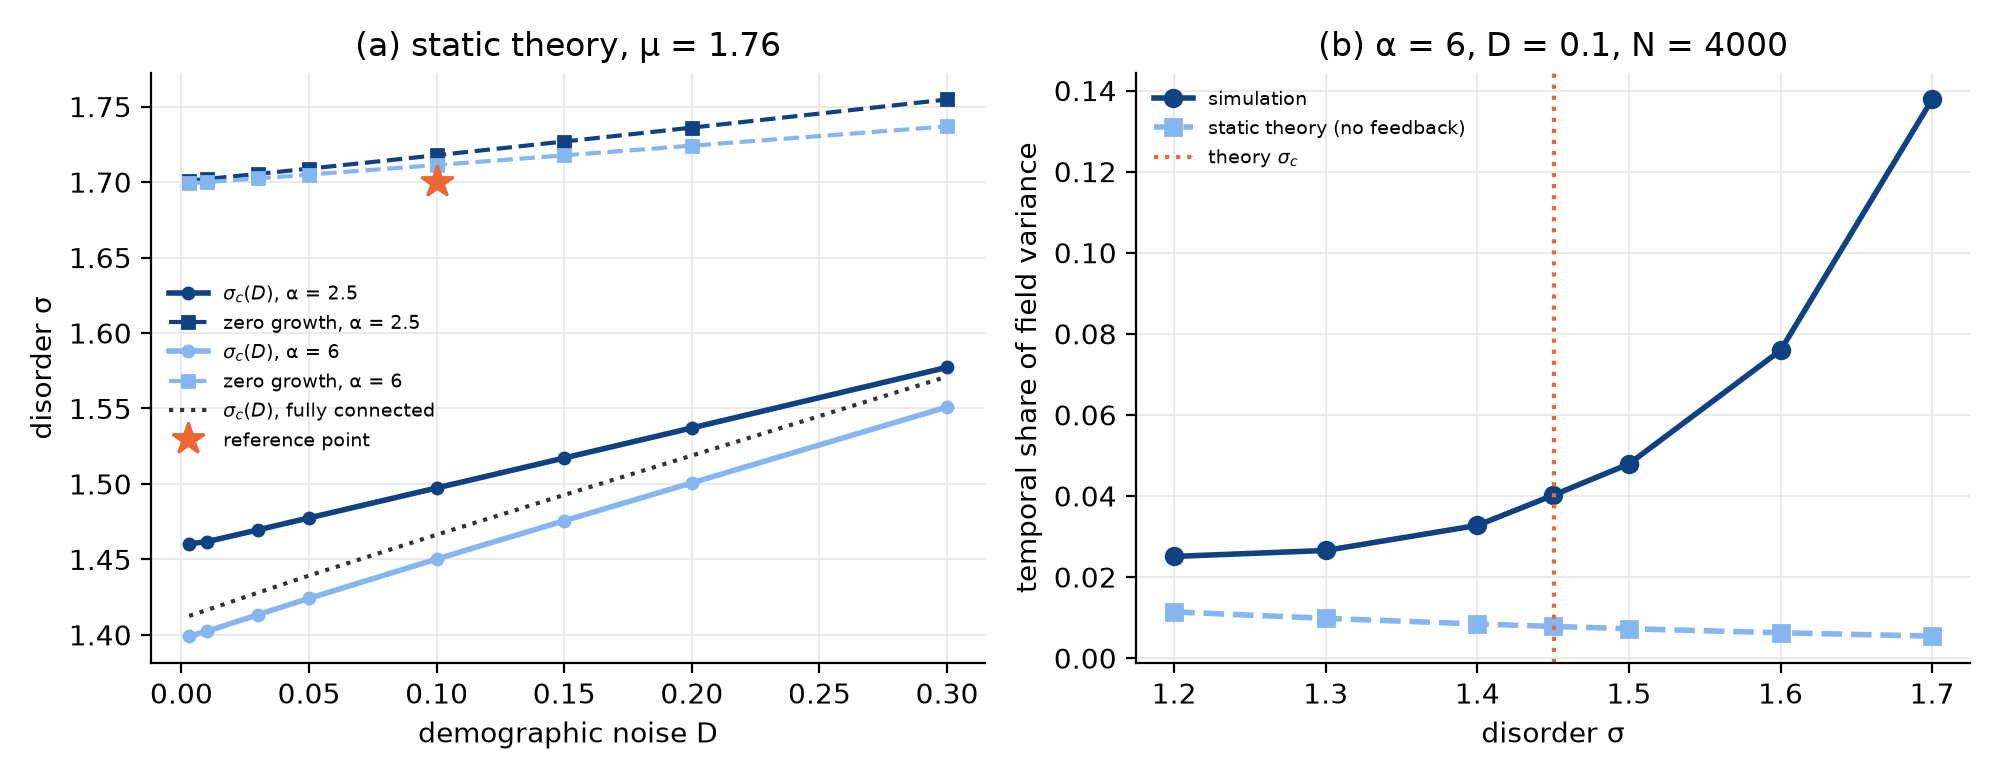
\includegraphics[width=\linewidth]{demographic_phase_lines.png}
\caption{(a) Static instability line $\sigma_c(D)$ and zero-growth line for two degree tails and the
fully connected graph, $\mu=1.76$; the star is the reference point.  (b) Temporal share of the field
variance in simulation and in the static closure, $\alpha=6$, $D=0.1$.}
\label{fig:phase}
\end{figure}

\paragraph{Turnover.}  The turnover rate barely depends on $D$: at $\sigma=1.75$ it is $0.64$ at
$D=0.003$ and $0.60$ at $D=0.3$ for $\alpha=2.5$, and $0.71$--$0.72$ for $\alpha=6$.  It is set by the
nodes with $h<0$, where a newborn's life does not depend on $D$ (Sec.~\ref{sec:constant}), and by the
fraction of such nodes, which depends on $\sigma$.  This is why the disorder, not the noise, controls
how many firms live long enough to be measured (Table~\ref{tab:params}).

%======================================================================
\section{The volatility law}
\label{sec:law}

\paragraph{Decomposition.}  In logs, $y=\ln S$ obeys
$dy=(\Phi-S-D/2S)\,dt+\sqrt{D/S}\,dW$.  Write $y=y_F+\delta$, where $y_F$ solves the noise-free equation
$\dot y_F=\Phi-e^{y_F}$ from the same initial size.  To linear order $\delta$ relaxes at the local rate
$S$ and is driven by noise of variance $D/S$, which is Eq.~\eqref{eq:plateau} with $\Phi\to S$.
Treating the two parts as independent,
\begin{equation}
\Var g\simeq V_F+B,\qquad B=\Big\langle\frac{D}{S^2}\big(1-e^{-S\Delta t}\big)\Big\rangle_{\rm life},
\label{eq:law}
\end{equation}
where $V_F$ is the growth variance of $y_F$ and the average runs over the life.

\paragraph{Test.}  For the $56\,293$ lives with $n_{\min}=20$ of two full economies we compute $V_F$
by integrating the noise-free equation along each life's measured field, and $B$ from its sizes.
Equation~\eqref{eq:law} reproduces the measured volatility to within $5\%$ over a decade and a
half of $\Sb$, and $9\%$ in the lowest bin (Table~\ref{tab:law}, Fig.~\ref{fig:law}).  A version
without the filter, $\Var(\Delta\ln\Phi)+D\Delta t\langle1/S\rangle$, overestimates by a near-constant factor
$1.47$: a firm does not follow the fast part of its field.

\begin{table}[b]
\caption{Volatility law \eqref{eq:law}, lives with $n_{\min}=20$, by deciles of $\Sb$
(selected rows).  Source: \texttt{scripts/demographic/volatility\_law.py}.}
\label{tab:law}
\begin{ruledtabular}
\begin{tabular}{cccccc}
$\Sb$ & sd$(g)$ & $\sqrt{V_F+B}$ & ratio & $\sqrt{V_F}$ & $\sqrt B$\\
\hline
0.19 & 0.742 & 0.809 & 1.09 & 0.253 & 0.769\\
0.47 & 0.635 & 0.630 & 0.99 & 0.296 & 0.556\\
0.91 & 0.561 & 0.540 & 0.96 & 0.315 & 0.438\\
1.39 & 0.512 & 0.492 & 0.96 & 0.319 & 0.374\\
1.85 & 0.470 & 0.444 & 0.94 & 0.312 & 0.317\\
3.59 & 0.373 & 0.353 & 0.95 & 0.273 & 0.223\\
\end{tabular}
\end{ruledtabular}
\end{table}

\begin{figure}[t]
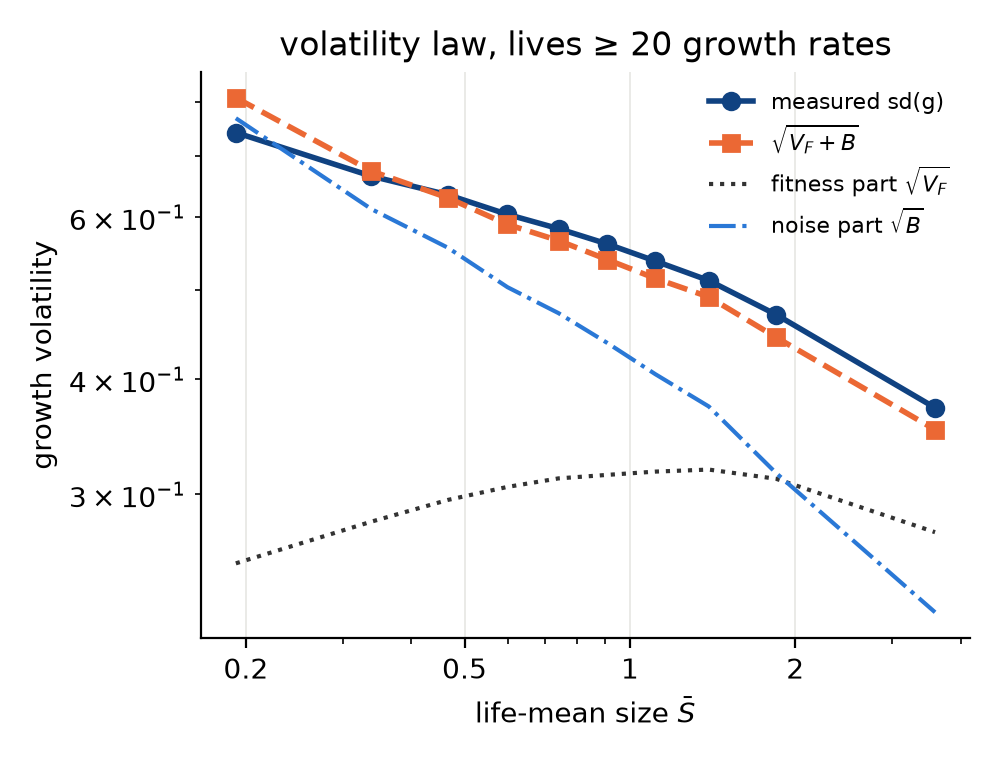
\includegraphics[width=0.85\linewidth]{demographic_volatility_law.png}
\caption{Volatility law \eqref{eq:law}: measured growth volatility, prediction, and its fitness and
demographic parts, by decile of life-mean size.}
\label{fig:law}
\end{figure}

\paragraph{Two regimes.}  The fitness part is nearly flat, $\sqrt{V_F}\simeq0.25$--$0.32$: competition
moves established firms by about the same amount whatever their size.  The demographic part falls
as $\langle S^{-1}\rangle^{1/2}$ for slowly relaxing firms and faster for large ones.  The size--volatility
relation is therefore a crossover,
\begin{equation}
v^2(\Sb)\simeq v_F^2+B(\Sb),
\label{eq:crossover}
\end{equation}
from a demographic regime with slope $-1/2$ to a fitness regime with slope $0$.  The two parts
are equal at $\Sb_\times\simeq1.9$ (Table~\ref{tab:law}).  The naive estimate
$\Sb_\times\approx D\Delta t/v_F^2\approx0.5$ is too small because $B$ is dominated by the low-size
excursions of a life, $\langle1/S\rangle\gg1/\Sb$.  Over $\Sb\in[0.19,3.6]$ the measured local slope is
$0.22$ and Eq.~\eqref{eq:crossover} gives $0.27$.

\paragraph{Dependence on $D$.}  A larger $D$ widens the demographic regime and moves the crossover
to larger sizes, so the effective exponent should grow with $D$.  It does: at $\alpha=2.5$,
$\sigma=1.75$, $n_{\min}=10$, $\beta=0.16$, $0.22$, $0.25$ for $D=0.05$, $0.1$, $0.15$
\todo{derive $\beta(D)$ from Eq.~\eqref{eq:crossover}}.

\paragraph{The fitness part.}  We do not yet have a formula for $v_F$.  The field keeps the
correlation shape $(1+|L|/\tau)e^{-|L|/\tau}$ of the deterministic model, with $\tau=1.42$ instead of about
$3.5$, and only $4\%$ of its variance is fast.  Linear response of the logistic filter predicts
$V_F$ falling with size, from $0.23$--$0.38$ to $0.14$--$0.15$, while the measured $\sqrt{V_F}$ is flat.
Large firms ride their plateau $S\simeq\Phi(t)$ with large relative swings of the field, and small
established firms spend up to $37\%$ of their steps with $\Phi<0$, so the response is nonlinear.  A
semi-analytic route is to drive one noise-free firm with a Gaussian field of the measured mean,
amplitude and $\tau$ in each degree class and average its growth variance.

%======================================================================
\section{The life panel}
\label{sec:panel}

\paragraph{Reference point.}  At $\alpha=2.5$, $\sigma=1.75$, $D=0.1$ the long lives give a nearly
straight decline (Fig.~\ref{fig:panel}).  At $N=32000$ with $C=200$:
\begin{center}\small
\begin{tabular}{cccc}
\toprule
$n_{\min}$ & $\beta$ & $\zeta_q/\zeta_1$ & decades\\
\midrule
2  & 0.13 & 2.53, 4.23, 5.94 & 2.2\\
5  & 0.16 & 1.90, 2.63, 3.18 & 2.0\\
10 & 0.16 & 1.76, 2.28, 2.58 & 1.8\\
20 & 0.20 & 1.77, 2.33, 2.71 & 1.4\\
\bottomrule
\end{tabular}
\end{center}
The spread of $\beta$ between economies is about $\pm0.035$.  For $n_{\min}=20$ the local exponents
over fifths of the range are $0.15$, $0.19$, $0.23$, $0.24$, $0.16$, so the curve flattens slightly at
the top, as the data do.  For $n_{\min}\ge5$ the exponent is in the empirical range and the ratio
curve bends below the line $\zeta_q=q\zeta_1$, slightly more than in Compustat.  For $n_{\min}=2$ the
ratios lie above that line.

\begin{figure*}[t]
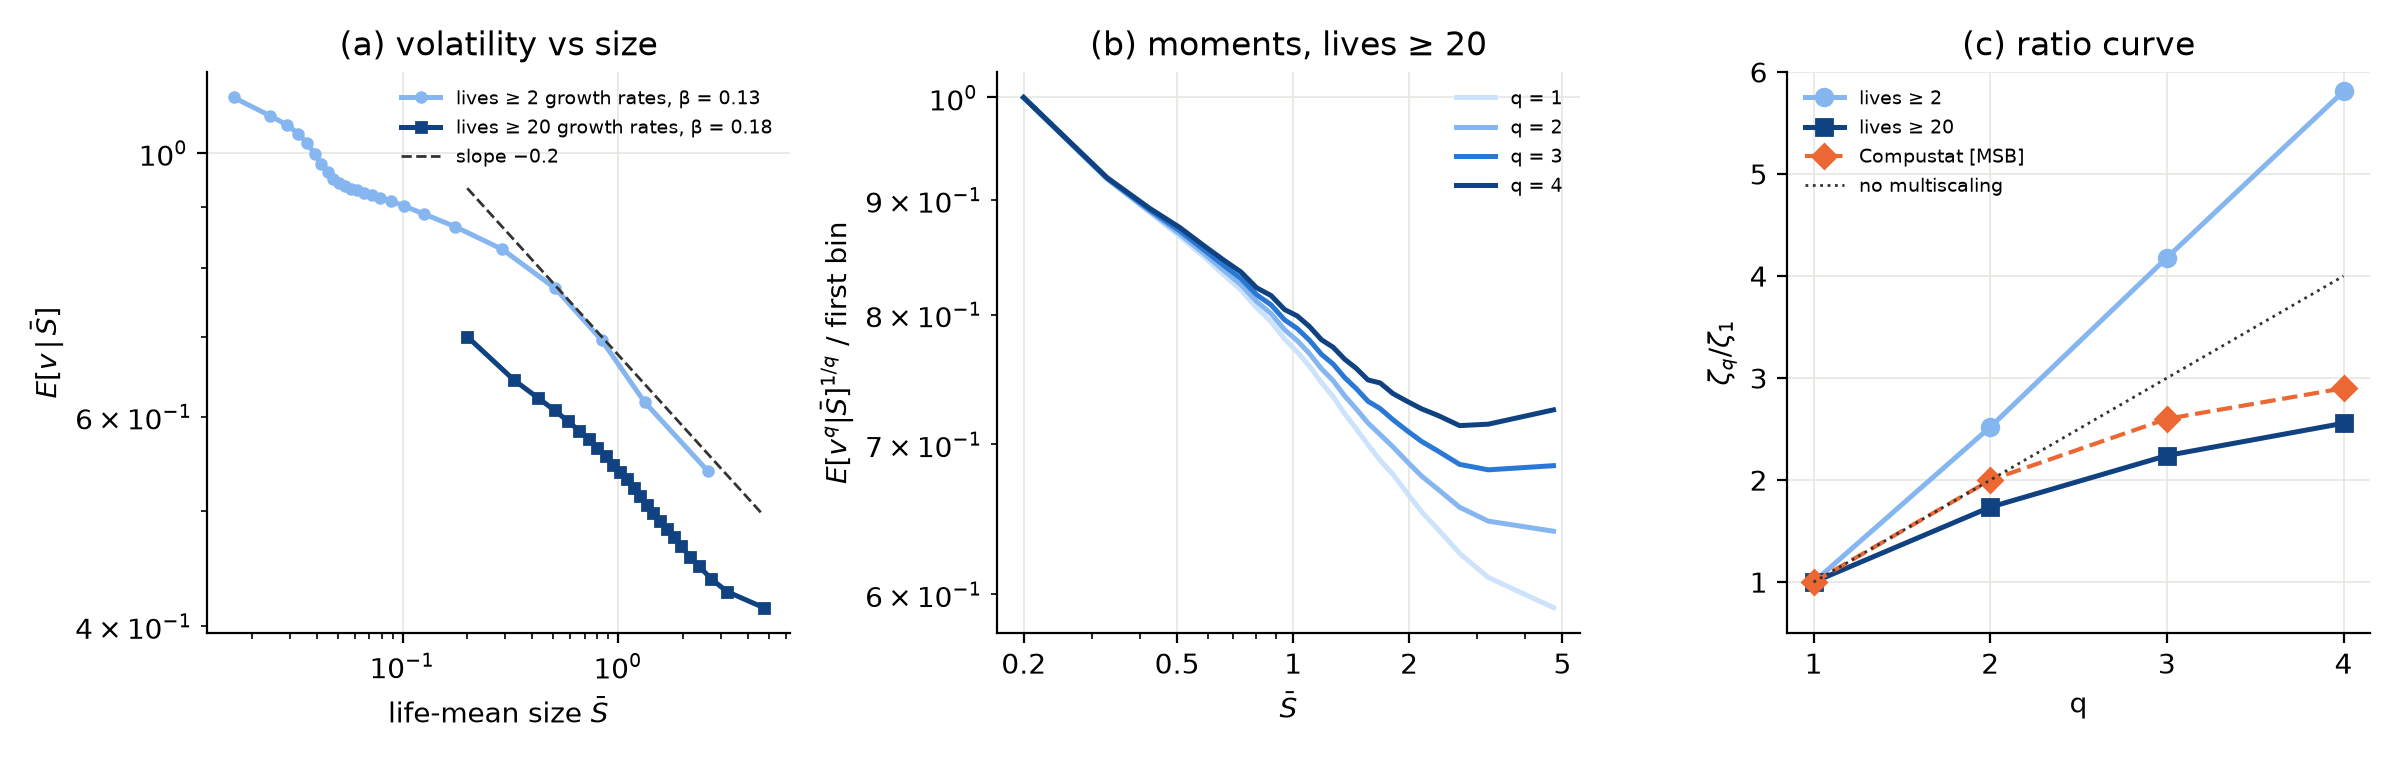
\includegraphics[width=\linewidth]{demographic_life_panel.png}
\caption{Life panel at the reference point ($\alpha=2.5$, $\sigma=1.75$, $D=0.1$, $N=32000$, $C=200$,
eight economies pooled).  (a) Mean volatility against life-mean size.  (b) Moments $q=1$--$4$
for $n_{\min}=20$.  (c) Ratio curves against Compustat \cite{moran2024}.}
\label{fig:panel}
\end{figure*}

\paragraph{Finite size.}  At $\alpha=2.5$ the configuration graph is saturated at $N=8000$, $C=200$:
merging multi-edges removes $40\%$ of edge ends and the largest hubs keep less than half their
intended degree.  At $N=32000$ the loss is $16\%$.  The shape survives the larger graph and
$\beta$ drops by $0.03$--$0.07$ (at $N=8000$: $0.17$, $0.20$, $0.22$, $0.27$).

\paragraph{Other parameters.}  Table~\ref{tab:params} collects the scan.  Three patterns are
robust.  (i) At $\alpha=6$ the long lives show a flat curve that plunges at the top, with
local exponents rising to about $1$; heavier degree tails are needed for a straight decline.
(ii) At small $D$ the long lives show a flat stretch or a hump, the gap between the demographic
regime and the plateau.  (iii) The disorder $\sigma$ sets the level of $\beta$ and the shape: at
$\sigma=1.6$ the top plunges again, at $\sigma=1.9$ turnover is so fast that volatility no longer
depends on size.

\begin{table}[b]
\caption{Scan at $N=8000$, $n_{\min}=20$.  Shapes: S, nearly straight; P, flat then plunging at the top;
H, rising at the bottom.  Source: \texttt{scripts/demographic/batch.py summary}.}
\label{tab:params}
\begin{ruledtabular}
\begin{tabular}{lllcc}
$\alpha$ & $\sigma$ & $D$ & $\beta$, $\zeta_q/\zeta_1$ & shape\\
\hline
6   & 1.75 & 0.001 & 0.15; 1.83, 2.48, 2.97 & P\\
6   & 1.75 & 0.1   & 0.40; 1.93, 2.77, 3.51 & P\\
3.5 & 1.9  & 0.001 & 0.08; 1.71, 2.15, 2.37 & H\\
3.5 & 1.9  & 0.1   & 0.20; 1.86, 2.57, 3.15 & S\\
3.5 & 1.9  & 0.3   & 0.29; 1.91, 2.71, 3.41 & S\\
3   & 1.9  & 0.1   & 0.15; 1.83, 2.49, 3.00 & S\\
2.5 & 1.75 & 0.05  & 0.21; 1.72, 2.20, 2.50 & S\\
2.5 & 1.75 & 0.1   & 0.27; 1.80, 2.39, 2.80 & S\\
2.5 & 1.6  & 0.1   & 0.46; 1.91, 2.71, 3.37 & P\\
2.5 & 1.9  & 0.1   & 0.07; 1.63, 1.93, 1.93 & flat\\
\end{tabular}
\end{ruledtabular}
\end{table}

\paragraph{Range.}  The decline of the long lives spans at most about two decades, from a few
times $D$ to the plateau.  A life must climb well above $D$ to last: in the demographic regime the
log-variance accumulated over a life is of order one (the exit time from size $S_0$ at $\Phi\approx0$
is of order $S_0/D$), so a firm whose growth is dominated by noise lives about $1/v^2$ growth
periods.  Below a few times $D$ only short lives exist.  Between $D$ and the plateau the dynamics are
Gibrat-like, $d\ln S/dt\simeq\Phi$, and only the two crossovers of Eq.~\eqref{eq:crossover} produce a size
dependence.  At $D=0.1$ they overlap and blend into one decline; at $D=10^{-3}$ they separate and
leave a flat stretch.

\paragraph{Current size.}  Conditioning on current size, with all firms, the reference point gives
$\beta=0.29$ but ratios $2.22$, $3.53$, $4.77$, above the line $\zeta_q=q\zeta_1$.

%======================================================================
\section{Other stylised facts and limits}
\label{sec:limits}

Figure~\ref{fig:facts} shows the other facts at the reference point (two economies, $N=8000$).

\begin{figure*}[t]
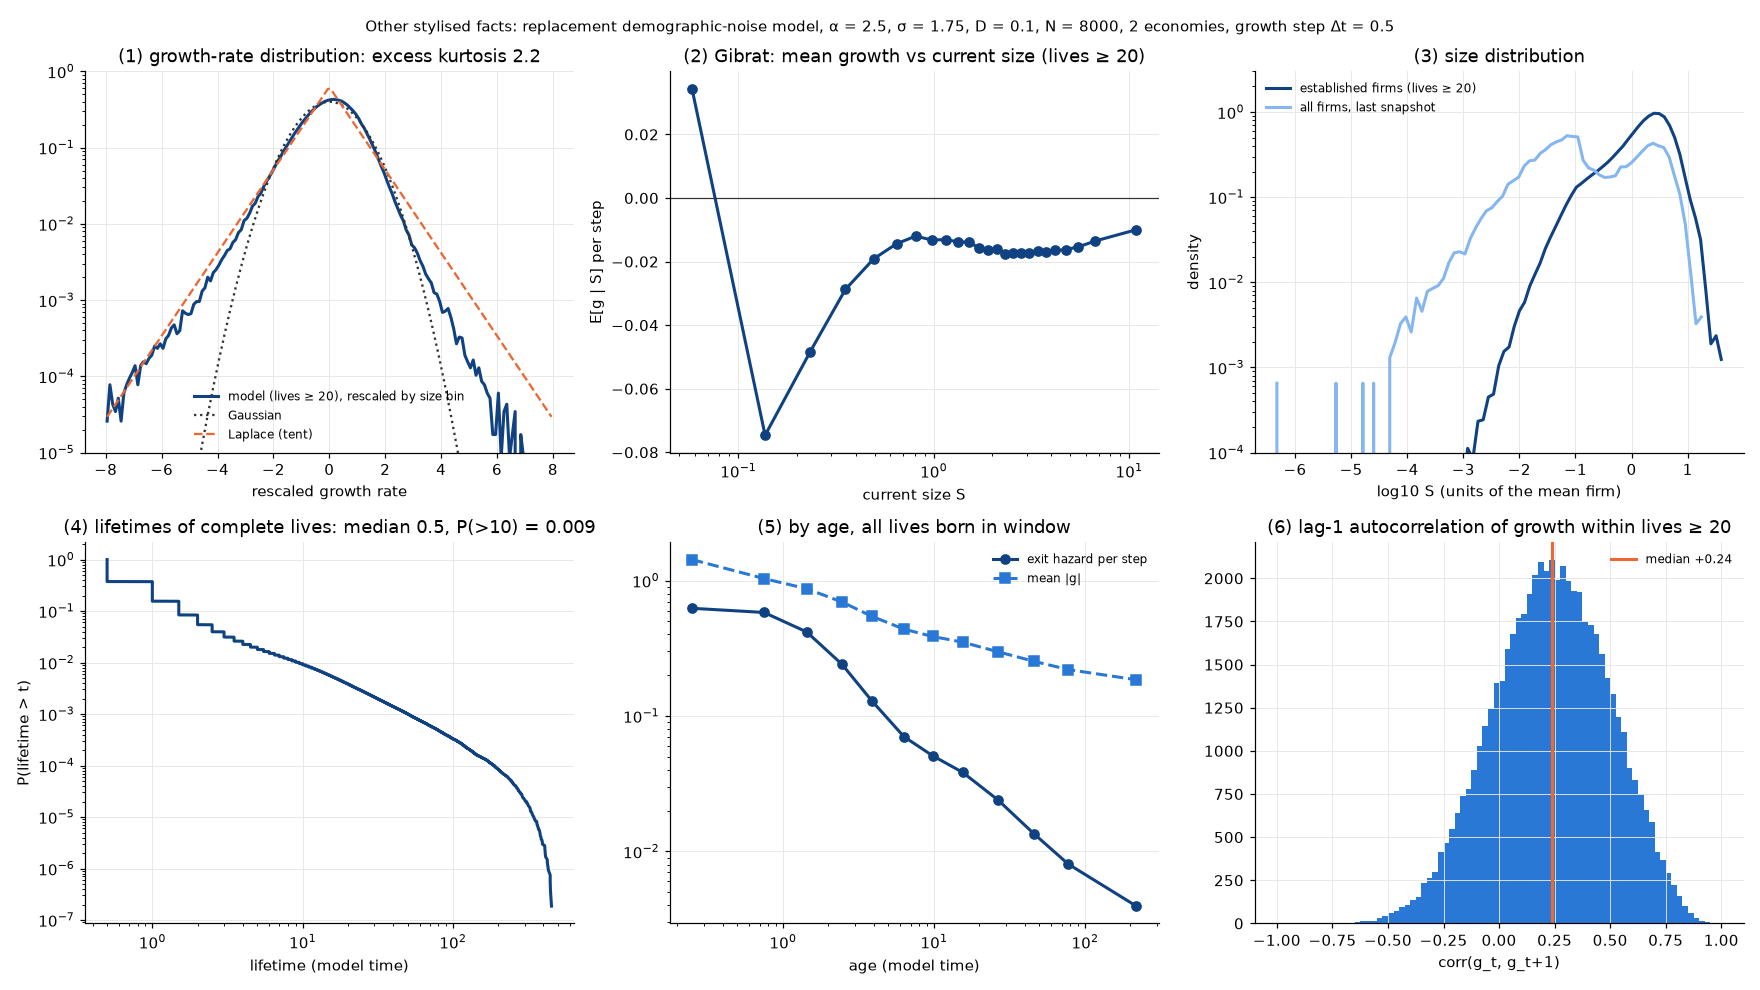
\includegraphics[width=0.9\linewidth]{demographic_facts.png}
\caption{Other stylised facts at the reference point.  (1) Growth rates of lives with
$n_{\min}=20$, rescaled by size bin.  (2) Mean growth against current size.  (3) Size
distributions.  (4) Lifetimes of complete lives.  (5) Exit hazard and mean $|g|$ against age.
(6) Lag-one autocorrelation of growth within lives.}
\label{fig:facts}
\end{figure*}

\paragraph{What holds.}  Growth rates are fat-tailed, with excess kurtosis $2.2$ (Laplace: $3$).
Mean growth is independent of size above about half the mean firm.  The exit hazard falls with age,
from $0.62$ per step at birth to $0.004$ for the oldest firms, and the mean $|g|$ falls from $1.4$ to
$0.19$; exits are concentrated in the smallest $70\%$ of sizes.

\paragraph{What fails.}
\begin{itemize}
\item \emph{Size distribution.}  Over all firms it is bimodal, with a newborn mode at $D$ and a plateau
  mode at a few times the mean.  Established firms have a left-skewed distribution
  ($\log_{10}$ standard deviation $0.54$, skewness $-0.97$) cut off at about ten times the mean.
  There is no Pareto tail \cite{axtell2001}.
\item \emph{Infant mortality.}  The median life is one sampling step; $0.9\%$ of lives exceed $10$
  time units.
\item \emph{Skewness.}  The left tail of the growth distribution is tent-shaped, the right tail close to
  Gaussian (skewness $-0.45$).  Large drops are firms on their way out.
\item \emph{Persistence.}  The lag-one autocorrelation of growth is $+0.24$ at $\Delta t=0.5$; it depends on
  how a sampling step maps to a year.
\item \emph{Small established firms} shrink on average (mean growth $-0.03$ to $-0.07$ per step near
  $S\approx0.1$--$0.3$), while in the data surviving small firms grow faster.
\end{itemize}

\paragraph{The plateau trade-off.}  The logistic term $-x_i/m$ does two jobs.  It bounds a firm with a
persistently favourable field, which keeps the economy from condensing, and its damping produces
the fitness floor of Eq.~\eqref{eq:crossover}.  Both require the plateau, and the plateau excludes a
Pareto tail.  Removing the term makes growth Gibrat-like, the condition under which a lower barrier
gives Zipf's law \cite{gabaix1999}, but here the quenched part of the field is not removed: in a test
at $N=4000$ the largest firm holds $95\%$ of the economy with the floor $\lambda$ and $88\%$ with
turnover, and volatility no longer depends on size.

\paragraph{A variant.}  Writing the noise directly in log size, $d\ln S=(\ldots)\,dt+\sqrt{D/S}\,dW$ without the
It\^o drag, is equivalent to the floor $\lambda=D/2$ plus square-root noise.  Exit is then impossible
and small firms are volatile and long-lived.  Conditioning on current size this variant gives
$\beta=0.21$--$0.35$ over five decades and ratios close to the data ($1.85$, $2.54$, $3.08$ at $\alpha=2.5$,
$D=0.002$), but the curve is a staircase and the spell panel returns to the hump of the
deterministic model.  Neither variant passes both protocols.

\paragraph{Interpretation of $D$.}  The noise unit $Dm$ grows with the mean firm.  It reads as a
firm's indivisible unit (a customer, a contract) growing with the economy, which is defensible
but not obvious.  At the reference point newborns enter at $10\%$ of the mean firm, larger than
real entrants relative to the mean.

%======================================================================
\section{Discussion}

Demographic noise turns the humped size--volatility curve of the deterministic Lotka--Volterra
economy into a monotone crossover.  The theory is a one-firm problem: a logistic unit driven by a
Gaussian field and by its own birth--death noise, exactly solvable at constant field, with a
volatility law that separates a size-independent fitness floor from a demographic part falling
as the inverse size.  Read this way, $\beta\approx0.2$ is the effective slope of a crossover between
slopes $-1/2$ and $0$ rather than a scaling exponent.  That is the shape Fontanelli et
al.\ \cite{fontanelli2025} report, and it predicts a crossover scale set by $D$ and $v_F$.  It is
harder to reconcile with a single power law over four decades \cite{moran2024}: the model's
straight stretch spans about two.

The model gives up the size distribution.  The plateau that produces the fitness floor also
caps firms at a few times the mean, and removing it condenses the economy.  A model that keeps
the law and recovers a Pareto tail needs a size dependence below the plateau that does not fix a
size scale, or persistent advantages that are not quenched.

\paragraph{Open problems.}
\begin{enumerate}
\item A formula for $v_F$ from the nonlinear one-firm problem in each degree class.
\item The two-time theory with demographic noise and turnover: the field's correlation above
  $\sigma_c(D)$, its collective amplification below it, and the fitness law (mean, amplitude and
  correlation time of $\Phi$ by degree) that the life panel needs.  Ref.~\cite{altieri2021} treats the
  static problem for symmetric couplings.
\item $\beta(D)$ and the ratio curve from Eq.~\eqref{eq:crossover} averaged over the distribution of lives.
\item The dependence of $\beta$ on $n_{\min}$ ($0.13$ to $0.20$), which MSB report to be weak in the data.
\item Empirical tests: the slope $-1/2$ regime and the crossover scale in data that include small
  firms, and the dependence of the measured exponent on how short-lived firms are filtered.
\end{enumerate}

\bibliography{../../bib,refs}

\end{document}
